
\frame{\titlepage}
\begin{frame}{}
    \centering
    \LARGE
    Introduction
    \end{frame}

\begin{frame}{Foundation Model's Context Length is growing rapidly}
    \begin{figure}
        \centering
        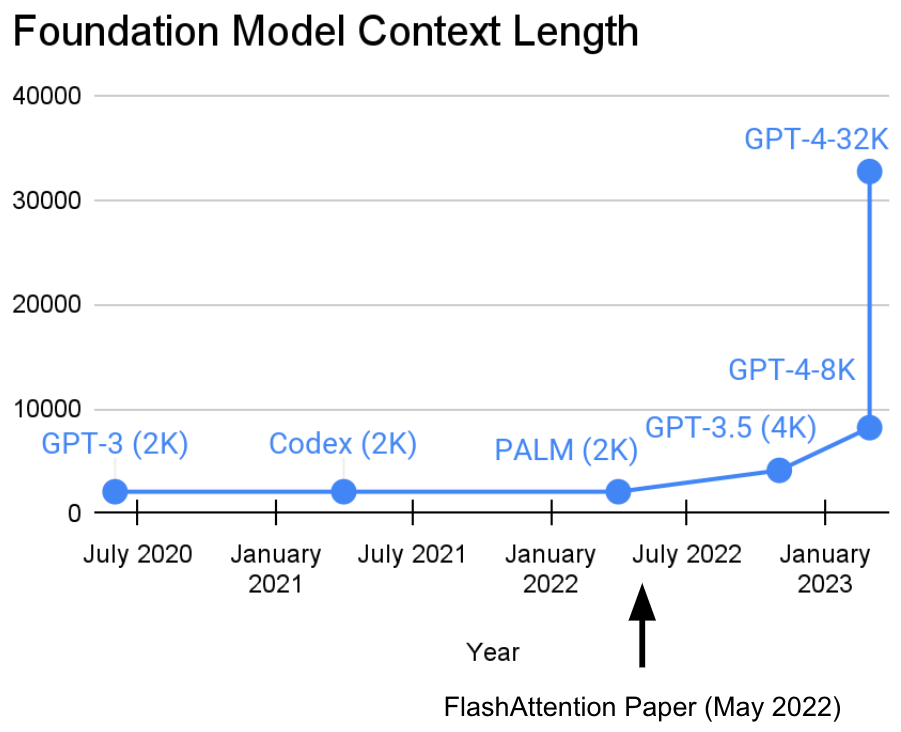
\includegraphics[width=0.75\linewidth]{figure/context.png}
    \end{figure}
\end{frame}

\begin{frame}{Issues with Transformers}

    \begin{itemize}
        \item Training: quadratic time complexity 
        \begin{itemize}
            \item Expensive for long sequence modeling (e.g., video or DNA modeling)
         \end{itemize}
        \item Inference: linear memory complexity
        \begin{itemize}
            \item Requires storing KV cache for each token
            \item High memory burden.
        \end{itemize}
    \end{itemize}    

\end{frame}

\begin{frame}{Revisiting RNNs}
    \begin{figure}
        \centering
        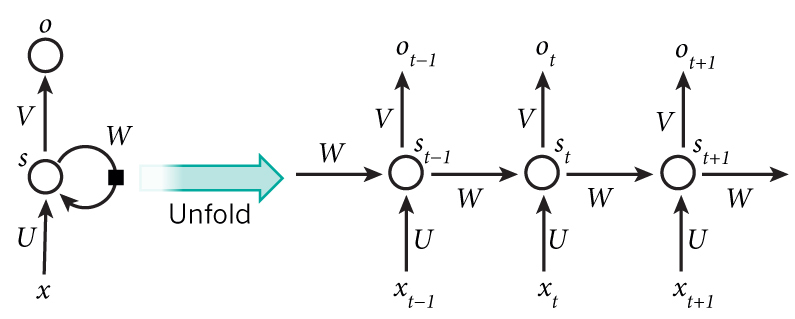
\includegraphics[width=.75\linewidth]{figure/rnn.png}
    \end{figure}
    \begin{itemize}
            \item Training: linear complexity, however, traditional RNNs are not parallelizable.
            \vspace{2mm}
            \item Inference: constant memory
    \end{itemize}
\end{frame}


\begin{frame}{Modern linear recurrent models}
    Use linear recurrence for parallel training
    \vspace{2mm}
    \begin{itemize}
        \item Gated linear RNNs (HGRN, Griffin, ...)
        \item State-space models (S4, Mamba, ...)
        \item Linear attention (RetNet, GLA, xLSTM, DeltaNet, ...)
    \end{itemize}

\end{frame}


\begin{frame}{Modern linear recurrent models}
    Use linear recurrence for parallel training
    \vspace{2mm}
    \begin{itemize}
        \item \textcolor{gray}{Gated linear RNNs (HGRN, Griffin, ...)}
        \item \textcolor{gray}{State-space models (S4, Mamba, ...)}
        \item \color{red}\textbf{Linear attention (RetNet, GLA, xLSTM, DeltaNet, ...)}
    \end{itemize}
    \vspace{2mm}
    \textcolor{black}{Linear attention is the focus of this talk.}
\end{frame}


\begin{frame}{}
    \begin{figure}
        \centering
        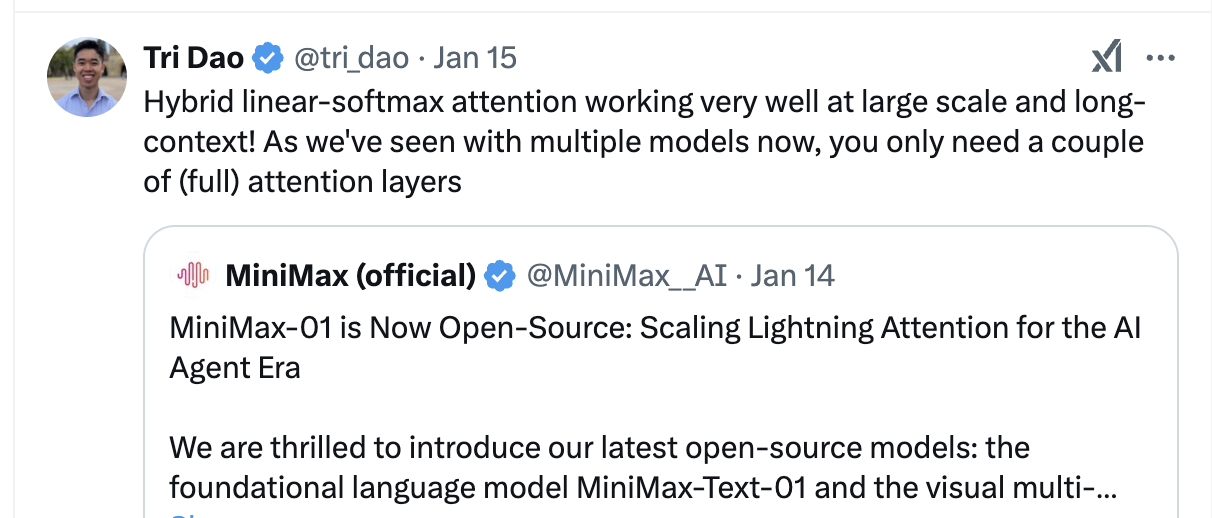
\includegraphics[width=.95\linewidth]{figure/hybrid_twitter.png}
    \end{figure}
    
    MiniMax-01 (\cite{minimax2025minimax01scalingfoundationmodels}) used hybrid attention: \textcolor{red}{\textbf{7/8}} linear attention layers + \textcolor{red}{\textbf{1/8}} softmax attention layers, with simple linear attention using data-independent decay: Lightning-Attention (\cite{Qin2024VariousLC}).
\end{frame}


